\documentclass[UTF8]{beamer} 
\usepackage{ctex}
\usepackage{Sweave}
\usetheme{Boadilla} 
\usepackage{color} 
\usepackage{graphicx} 

\begin{document}


\title{R编程与进化分析} 
\subtitle{第二部分 参数估计与进化树推断}
\author{张金龙} 
\institute{jinlongzhang01@gmail.com}
\date{2016年5月9日 北京} 

\frame{\titlepage} 

\begin{frame}
\frametitle{目录}
\tableofcontents
\end{frame}


\section{从线性模型说起}

\begin{frame}
\frametitle{目录}
\tableofcontents[currentsection] 
\end{frame}

\frame{
    \frametitle{线性回归}
\begin{block}{lm的应用}
{\tt set.seed(12345)\\
x = 1:40 + 3*rnorm(40)\\
y = 1:40 + rnorm(40)\\
dat $<-$ data.frame(x, y)\\
plot(y $\sim$ x, data = dat)\\
lmodel $<-$ lm(y $\sim$ x)\\
summary(lmodel)\\
abline(lmodel, col = 2)\\
text(10, 35, "Adjusted expression(R$\wedge$2) = 0.9258")}\\
\end{block}
}

\frame{
    \frametitle{AIC: Akaike Information Criterion}
日本统计学家赤池弘次在1971年提出赤池系数用来
权衡所估计模型的复杂度和该模型拟合数据的优良性。\\
寻找可以最好地解释数据但包含最少参数的模型。\\
假设条件为模型的误差服从独立正态分布。\\
让n为观察数,RSS为剩余平方和,那么AIC变为:\\
\[AIC = 2k+n\*ln(RSS/n)\]
更一般的AIC,
\[AIC = 2k-2ln(LogLik)\]
}

\frame{
    \frametitle{多个变量的逐步回归举例}
在变量较多的情况下, 常常需要将影响不显著的变量剔除出模型, 此时就涉及到多个模型比较的问题。 

\begin{block}{逐步回归举例}
{\tt cement$<-$data.frame(\\
X1=c( 7, 1, 11, 11, 7, 11, 3, 1, 2, 21, 1, 11, 10),\\
X2=c(26, 29, 56, 31, 52, 55, 71, 31, 54, 47, 40, 66, 68),\\
X3=c( 6, 15, 8, 8, 6, 9, 17, 22, 18, 4, 23, 9, 8),\\
X4=c(60, 52, 20, 47, 33, 22, 6, 44, 22, 26, 34, 12, 12),\\
Y =c(78.5, 74.3, 104.3, 87.6, 95.9, 109.2, 102.7, 72.5,\\
93.1,115.9, 83.8, 113.3, 109.4))\\
lm.sol$<-$lm(Y $\sim$ X1+X2+X3+X4, data=cement)\\
summary(lm.sol)\\
lm.step$<-$step(lm.sol)\\
summary(lm.step)}\\
\end{block}
}

\frame{
    \frametitle{pairs查看多个变量的分布}

pairs() 用来查看多元变量\\
从pairs进一步衍生出诸如hydropairs\\
 \begin{center}
    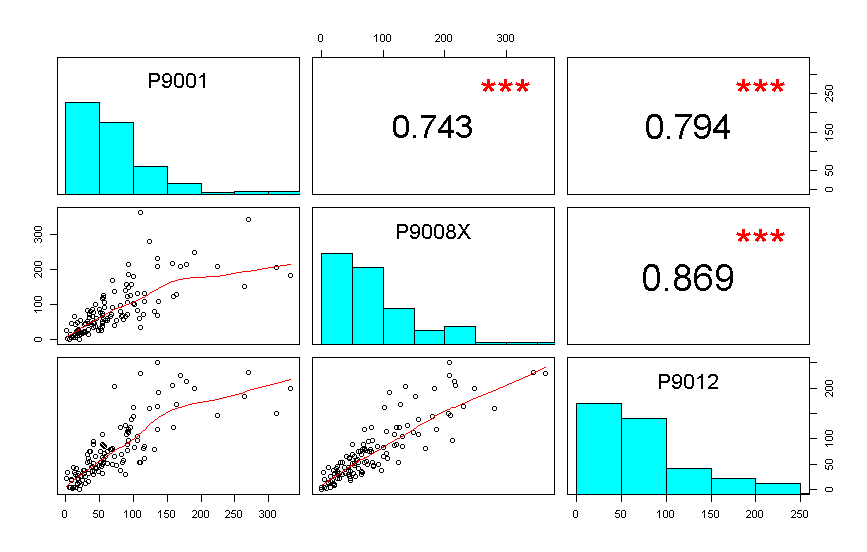
\includegraphics[height=2.in]{hydropairs.png}\\
    \medskip
   hydroTSM的hydropairs\\
    \end{center}
图中的趋势线, 用lowess()函数获得\\

}



\section{极大似然估计 Maximum Likelihood}
\begin{frame}
\frametitle{目录}
\tableofcontents[currentsection] 
\end{frame}


\frame{
    \frametitle{黑球白球的比例问题}
现在假设一个袋子里有100个球, 黑白若干。 随机从中抽取了20个, 其中有15个黑球, 5个白球, 问: 袋子里面, 黑球和白球各占的比例, 最可能是多少?\\
参数的取值应该是什么, 才能最大可能性地获得当前的数据?这就是极大似然的思想。 \\
可以假设这100个球中, 黑球比例为p, 白球则为1-p, 抽取15个黑球, 为p$\wedge$15, 5个白球为(1-p)$\wedge$5, 当前的数据, 就是抽取到了15个黑球, 5个白球, 这些事件同时发生了, 因此, 将每一个事件发生的概率相乘。 所以当前事件发生的概率为\\

Prob = p$\wedge$15*(1-p)$\wedge$5 \\
此时, Prob称为Likelihood, 其本质即为联合概率密度\\
}


\frame{
    \frametitle{似然公式}
极大似然法方法和概率公式相同, 不过这里概率密度的参数正式需要通过样本数据来估计的,是未知的, 而概率公式中, 概率是已知的。\\
已知正态分布的概率密度 \\
\[pdf(y) = \frac{1} {\sqrt{2 \pi} \sigma} e^{-1/2 \frac{(y- \mu)^2} {\sigma^2}}\]
假设数目取自一个正态分布总体,对所有的样本数据的概率密度相成, 即获得联合概率密度, 即似然函数。
似然函数为 \[L = pdf_1 * pdf_2 * pdf_3 * ... * pdf_n\]
}

\frame{
    \frametitle{Likelihood}

对于样本取自正态分布的样本, 其似然函数为:\\
\[L = \prod_{i=1}^n \frac{1} {\sqrt{2 \pi} \sigma} e^{-1/2 \frac{(y- \mu)^2} {\sigma^2}}\]
\begin{block}{正态分布数据的似然函数}
\tt{
like = function(data, mu, sigma) \{ \\
    like = 1 \\
    for(i in 1:length(data))\{ \\
    \# like = like *( 1/(sqrt(2*pi)*sigma) * exp(-1/2 * (data[i] - mu)$\wedge$ 2/(sigma $\wedge$ 2))) \#\#\# 本行和下一行任取其一即可。 \\
    like = like * dnorm(x = dat[i], mean = mu, sd = sigma) \\
\} \\
return(like) \\
\} \\
}
\end{block}
}

\frame{
    \frametitle{Log Likelihood}
由于一件事的发生(如样本数据), 是多个条件共同满足的结果, 而每个事件发生的概率又都可能较小, 一般情况下, Likelihood函数值都非常小。为了方便计算, 一般取自然对数log.这就是对数似然函数 Log Likelihood。\\
\begin{block}{对数似然函数R code}
\tt{
loglike = function(data, mu, sigma)\{ \\
loglike = 0\\
for(i in 1:length(data))\{\\
loglike = loglike + log(dnorm(x = dat{[i]}, mean = mu, sd = sigma))\\
\}\\
return(loglike)\\
\}\\
}
\end{block}

}



\frame{
    \frametitle{黑球白球比例的极大似然估计}
p值为多少, 才能够保证我们取出15个黑球,5个白球? \\
思路: 可以在一个区间内, 将p从大到小取值, 之后找到让Prob最大时, 所对应的p值。 \\
\begin{block}{}
{\tt
seqx $<-$ seq(0,1, by = 0.001)\\
Like $<-$ function(p)\{ p$\wedge$15*(1-p)$\wedge$5\\\} \#似然函数 \\
logLike $<-$ function(p)\{ log(p$\wedge$15*(1-p)$\wedge$5)\}\\ \#对数似然函数\\

Like.res $<-$ Like(seqx)\\
logLike.res $<-$ logLike(seqx)\\

par(mfrow = c(1, 2))\\
plot(Like.res $\sim$ seqx, type = "l", xlab = "p", ylab = "Likelihood")\\
plot(logLike.res $\sim$ seqx, type = "l", xlab = "p", ylab = "Log Likelihood")\\
}
\end{block}
}


\frame{
    \frametitle{黑球白球比例的极大似然估计}
为了求得满足极大似然的参数, 一般在R中, 返回值前面加一个负号, 这样求极大似然法, 就变为求函数最小值的问题。\\
logLike 也相应变为 MinuslogLike\\
\begin{block}{}
{\tt
MinuslogLike $<-$ function(p)\{\\
     return(-log(p$\wedge$15*(1-p)$\wedge$5))\\
\}\\
}
\end{block}
利用nlm函数, 求另外一个函数的最小值。p设定为一个初始值。nlm将进行迭代, 直到数值收敛到一个很小的范围内, 才会终止。\\
\begin{block}{}
{\tt
MLEst $<-$ nlm(f = MinuslogLike, p = 0.01)\\
}
\end{block}
}

\frame{
    \frametitle{Likelihood vs Log Likelihood}
    \begin{center}
    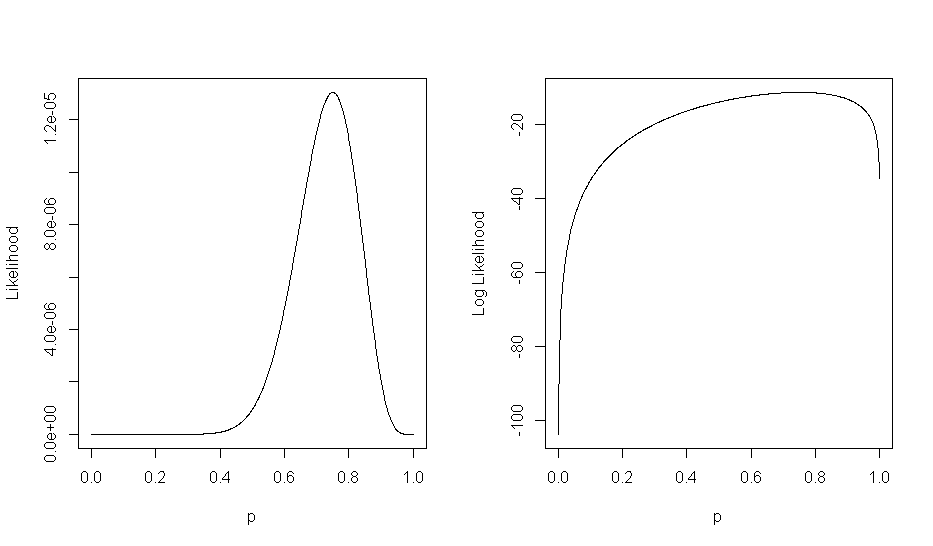
\includegraphics[height=2.5in]{likelihood2.png}\\
    \medskip
    Likelihood vs Log Likelihood\\
    \end{center}
}

\frame{
    \frametitle{极大似然估计举例}
数学中极大似然估计的求解过程:\\
\begin{itemize}

\item(1)写出似然函数;\\
\item(2)对似然函数取对数,并整理;\\
\item(3)求导数 ;\\
\item(4)解似然方程\\
\end{itemize}
计算机中, 求极大似然估计的过程\\
\begin{itemize}

\item(1) 写出对数似然函数的表达式\\
\item(2) 将返回值前加一个负号\\
\item(3) 用nlm函数, 求该函数的极小值。\\
\end{itemize}
}

\frame{
    \frametitle{线性模型的极大似然估计}
要了解响应变量y与因变量x之间的关系, 人们常用到线性回归。 常用 y = a*x + b表示, 然而更一般格式为

y = beta1*x + beta0 + error

其中beta0, beta1是参数,分别为截距和因变量的系数,error为残差。按照线性模型的假设, 残差应符合正态分布,一般取均值mean为0, 只需要估计标准差sd即可。
}


\frame{
    \frametitle{对线性模型进行极大似然估计的步骤}
(1) 生成要拟合的数据, 并绘图\\

(2) 通过R函数的内置lm方法建立线性模型, 并计算AIC以及LogLikelihood以便进行比较\\

(3) 建立对数似然函数 Log Likelihood\\

(4) 利用bbmle程序包的 mle2函数, 用数值优化算法(Optimization)求似然函数的最大值,从而给出所求参数的估计值。\\

(5) 基于最大对数似然值 Maximum Log Likelihood求该模型的AIC值(Akaike Information Criterion)\\
}


\frame{
    \frametitle{生成要拟合的数据}

\tt{ library(bbmle)  导入bbmle程序包

set.seed(12345)     设定随机数种子

x = 1:60        生成x数据, 共60个值

y = x*5 + 20 + rnorm(60, 0, 20) 生成y数据, 这里假设已知 beta1 = 5,  beta0 = 20, mu = 0, sd = 20
}
}


\frame{
    \frametitle{进行线性拟合以及计算LogLikelihood, AIC}
\tt{
 1. 绘图观察数据\\
plot(y ~ x, main = "Fitting of a Linear Model ")\\
2. 建立线性模型\\
linmod $<-$ lm(y ~ x) \\
3. 添加拟合直线\\
lines(x, fitted(linmod) , lty = 1, col = "red", lwd = 2)   \\
4. 添加残差线\\
segments(x0 = x, y0 = y, x1 = x, y1 = fitted(linmod)) \\
5. 查看模型的拟合参数\\
summary(linmod)  \\
6.  计算AIC Akaike Information Criterion\\
(AIC1 $<-$ AIC(linmod))  \\
7. 计算 Loglikelihood\\
(logLik1 $<-$ logLik(linmod)) \\
}
}


\frame{
    \frametitle{拟合线性模型, 残差正态分布}
    \begin{center}
    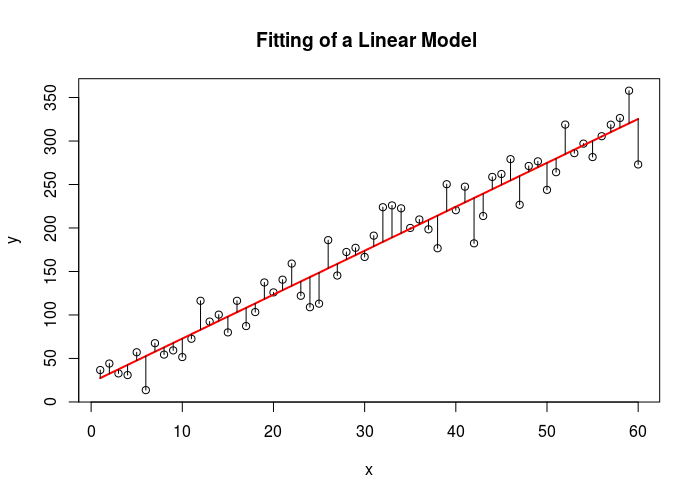
\includegraphics[height=3in]{Rplot06.png}\\
    \end{center}
}



\frame{
    \frametitle{线性模型的 Log Likelihood Function}
\tt{
函数的一般形式\\
y = beta1*x + beta0 + error\\
而error一项, 服从正态分布\\
所以 error = y - beta1*x - beta0\\
所以Loglikelihood函数可以写成如下形式:\\

LL $<-$ function(beta0, beta1, mu, sigma)\{\\
       R = y - x*beta1 - beta0  \\
       -sum(dnorm(R, mu, sigma, log = TRUE))\\
\}
}
}


\frame{
    \frametitle{线性模型的 Log Likelihood Function}
\tt{
 mle2函数, 可以用来估计似然函数取极值时,各参数的取值, 调用方式如下:\\
res $<-$ mle2(LL, start = list(beta0 = 1, beta1 = 2, mu = 1, sigma = 1), fixed = list(mu = 0))\\
summary(res)\\

因为mle2的结果是S4类型, 所以这里用@提取\\

基于参数估计,计算y2的取值\\
y2 $<-$ x*(res$@$coef[2]) + res$@$coef[1]\\

添加极大似然估计值\\
points(y2 ~ x, col= "blue", type = "b", pch = 19)\\
}
}

\frame{
    \frametitle{用极大似然法估计线性模型的参数}
    \begin{center}
    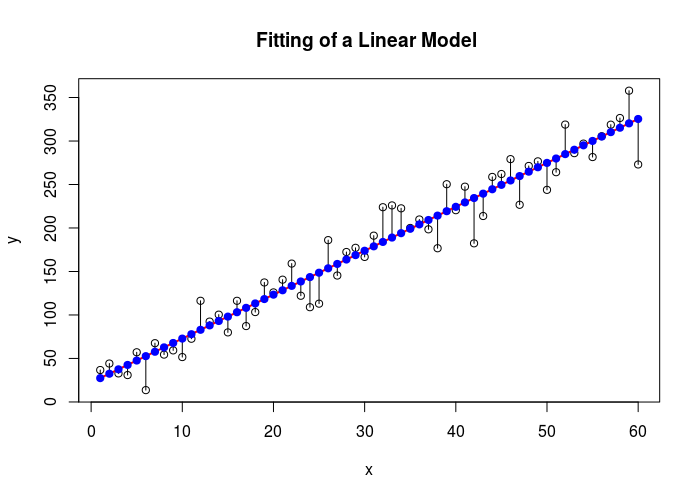
\includegraphics[height=3in]{Rplot07.png}\\
    \end{center}
}

\frame{
    \frametitle{线性模型的 Log Likelihood Function}
\tt{
 用mle2得出来的Maximum Log Likelihood\\
(logLik2 <- logLik(res))\\
计算AIC, 的公式为 AIC = -2*logLik + 2*p, 其中logLike为 Maximum Log Likelihood, p为参数的个数。\\
 因为在参数估计中, mu为一个常数0,我们只估计了sigma, 所以估计的参数是3个\\
(AIC2 = -2*logLik(res) + 2*3)\\

}}




\frame{
    \frametitle{最优化方法与参数估计}

在R中, 人们用多种优化方法, 求得极大似然估计的数值解。 这些方法包括 \\
\begin{block}{最优化方法}
"Nelder-Mead" (Nelder and Mead ,1965) \\
"BFGS" (Broyden, Fletcher, Goldfarb and Shanno, 1970)\\
"CG" (Fletcher and Reeves,1964) \\
"L-BFGS-B" (Byrd et. al. ,1995)  \\
"SANN" (Belisle 1992), 等。\\
\end{block}
用求得的Log Likelihood和模型参数的数量, 可以用来计算AIC。\\
}

\frame{
    \frametitle{极大似然估计在进化中的应用}
    \begin{itemize}
    \item 构建进化树,如 RAxML, PHYLIP, GARLI等
    \item 线性模型以及广义线性模型的参数估计 如 lme4
    \item 祖先状态重建: mesquite, ape
    \item 祖先分布区重建: Lagrange
    \item 分化时间推断: r8s
    \item 物种分化速率和灭绝速率的推断: laser, geiger, diversitree
    \end{itemize}
}

\section{贝叶斯统计基础}
\begin{frame}
\frametitle{目录}
\tableofcontents[currentsection] 
\end{frame}


\frame{
    \frametitle{频率学派和贝叶斯学派}
贝叶斯推断是参数估计的一种方法,但是贝叶斯推断不是估计出参数的固定值, 而是生成所估计参数的分布。\\
\textbf{频率学派}: 给定当前的假设,观察到当前的样本的概率是多少?\\
\begin{itemize}
\item 被估计的参数未知,但是有一个确定值;\\
\item 需要根据重复取样对概率分布进行客观取样;\\
\item 样本量越大,参数的估计就越准确;\\
\item 进行极大似然估计\\
\end{itemize}
\textbf{贝叶斯学派}:给定样本数据,待估计参数的概率分布如何?\\
\begin{itemize}
\item 待估计的参数是统计分布;\\
\item 主观得假设参数服从某种分布(先验分布);\\
\item 无需大样本;\\
\item 基于统计模拟, 对参数进行估计。\\
\end{itemize}
}

\frame{
    \frametitle{频率学派和贝叶斯学派}
    \begin{center}
    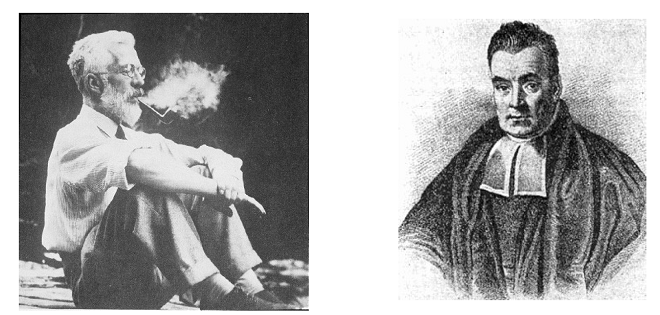
\includegraphics[height=2in]{bayes.png}\\
    \medskip
    Fisher 和 Bayes\\
    \end{center}
}

\frame{
    \frametitle{贝叶斯推断}
人们希望获得参数的概率密度分布, 而不仅仅是获得一个估计值。 人们对参数值取值数量的增多, 从而对参数分布有更深入了解, 其中体现了贝叶斯思想。 \\
\[p(\theta|y)=\frac{p(y|\theta)p(\theta)}{p(y)}\]
$\theta$是待估计的参数\\
$y$是样本数据\\
\textrm{$p(y|\theta)$是样本的概率密度(Likelihood)}\\
$p(\theta)$是主观假定的参数概率密度\\
$p(y)$是 Normalizing constant\\
\[p(y)=\int P(y|\theta)P(\theta)d\theta\]
即所有生成当前数据的概率相乘。很多情况下,$p(y)$是无法用表达式求出的。而是要用到MCMC的方法。\\
}


\frame{
    \frametitle{贝叶斯方法的优缺点}
贝叶斯方法的优点:
\begin{itemize}
\item 能够计算出待估计参数的概率分布;\\
\item 能够解决常规方法不能解决的复杂问题;\\
\end{itemize}
贝叶斯方法的缺陷:\\
\begin{itemize}
\item 需要高深的统计知识,难以理解;\\
\item 需要强大的计算能力;\\
\item 在指定参数的先验概率分布时,需要进行足够的解释;\\
\end{itemize}
一般用蒙特卡洛马尔科夫链Metropolis Coupling(Monte Carlo Markov Chain Metropolis
Coupling, MCMCMC, $MC^{3}$)的方法生成参数的分布。
}

\frame{
    \frametitle{马尔科夫链 Metropolis coupling}
\[p(y)=\int P(y|\theta)P(\theta)d\theta\]
由于贝叶斯公式难以获得解析解。在无法获得参数联合概率密度的情况下,蒙特卡罗马尔科夫链可以保证在后验分布的参数空间中取样,当获得大量后验分布的样本后,即可获得后验概率的近似分布。\\

某一事件在t时刻状态B的概率只与之前一个时刻t0的状态A有关,而与t0时刻之前的状态以及t之后的状态无关, 则称该过程具有马尔科夫性。\\
时间和状态都是离散的马尔科夫过程称为马尔科夫链。\\

Metropolis-Coupling为抽样策略的一种,还有一种限制性的Gibbs抽样法是Metropolis-Coupling的特例。\\
}


\frame{
    \frametitle{Metropolis-Coupling算法(Metropolis-Hasting)}
Metropolis Hasting(下面简称MH)是蒙特卡罗马尔科夫链中一种重要的抽样方法。\\
\begin{itemize}
\item MH算法在参数空间随机取值,作为起始点。
\item 按照参数的概率分布生成随机的参数,按照这一系列参数的组合,计算当前点的概率密度。\\
\item 依据当前点和起始点概率密度比值是否大于(0,1)之间的随机数来判断是否保留当前点。\\
\item 若当前点的概率密度大于该随机数,就称这种状态为接受状态,\\
\item 此时,在满足参数概率分布的前提下,继续随机抽取参数的组合,作为下一点,\\
\item 计算下一点的概率密度,并计算下一点概率密度和概率密度的比值,并继续循环。\\
\item 若当前点不能被接受,则继续在满足参数概率分布的前提下,继续生成随机数,作为新的参数组合,直到参数组合能够被接受为止。
\end{itemize}
}

\frame{
    \frametitle{Simulated Annealing}
    \begin{center}
    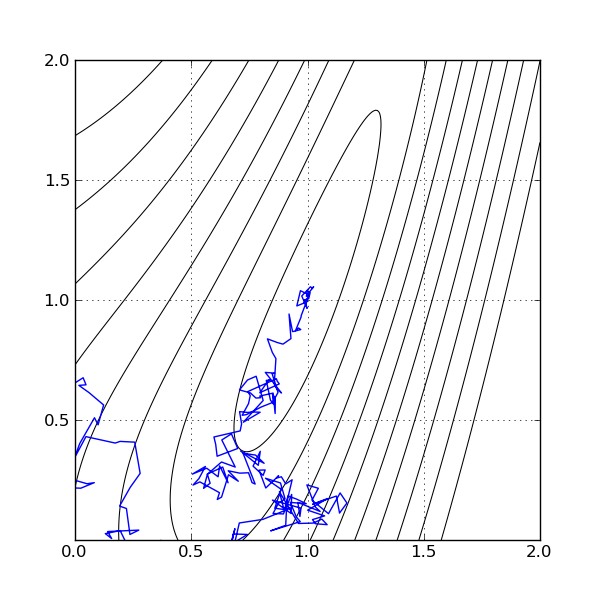
\includegraphics[height=2.6in]{continuous-simulated-annealing.png}\\
    \medskip
    二维参数空间上运行的马尔科夫链举例,等高线表示理论预测的概率密度, MCMCMC在接近多代后,生成接近理论预测的概率密度分布。\\
    \end{center}
}



\frame{
    \frametitle{冷链Hot Chain 和热链 Cold Chain}
\begin{itemize}
\item 参数随机改变的快慢,称为马尔科夫链的“温度”,变化越激烈,马尔科夫链越热。\\
\item 在实际情况中,往往设置若干条温度不同的马尔科夫链, 在参数空间中不断走动。\\
\item 参数变化较快的马尔科夫链,称为热链, 便于发现概率密度更高的区域。\\
\item  一旦发现概率密度更高的区域, 则冷热链交换, 冷链在概率密度更高的区域内走动,
热链则继续寻找概率密度更高的区域。
\end{itemize}
\begin{itemize}
\item 热链用于帮助马尔科夫链收敛 
\item 冷链用于精确样本的积累
\end{itemize}
}

\frame{
    \frametitle{冷链和热链}
    \begin{center}
    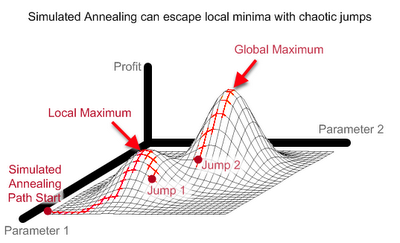
\includegraphics[height=2.3in]{mcmc.png}\\
    \medskip
在参数空间中,冷链取值变化范围小,移动较慢;热链取值变化范围大, 移动较快。 一旦热链发现概率密度更高的区域, 冷链, 热链交换。冷链热链的设置, 能够更快速形成符合概率密度分布的抽样。
    \end{center}
}


\frame{
    \frametitle{用MCMC的方法估计线性模型的参数}
    \tt{
第一步 首先生成要拟合的数据\\
设定随机数种子\\
set.seed(12345)\\     
生成x数据, 共60个点\\
x = 1\:60           \\
beta0真实值为20\\
beta0\_actual = 20\\   
beta1真实值为5\\
beta1\_actual = 5\\   
sigma真实值为15\\
sigma\_actual = 15\\  
y = x*5 + 20 + rnorm(60, 0, 15)  生成y数据, 这里假设已知 beta1 = 5, beta0 = 20, mu = 0, sd = 15\\

}
}

\frame{
    \frametitle{用MCMC的方法估计线性模型的参数}
      \begin{center}
    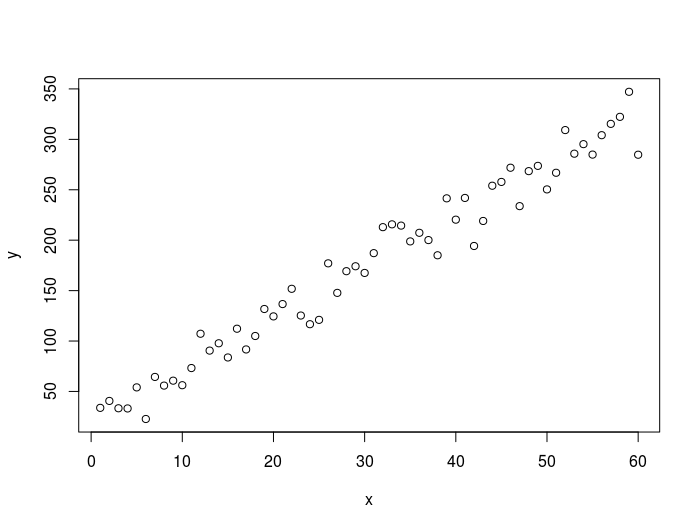
\includegraphics[height=2in]{Rplot08.png}\\
    \end{center}  
\tt{
plot(y ~ x)         绘图\\
本套模拟数据所应的 beta0, beta1\\
linmod $<-$ lm(y ~ x)\\
summary(linmod)\\
}
}

\frame{
    \frametitle{用MCMC的方法估计线性模型的参数}
    \tt{
第二步, 写出 似然函数, 因线性回归一般模式均可写成\\
    \medskip
y = beta1*x + beta0 + error,\\

其中的误差项error符合 N(0, sigma)\\
    \medskip
    \medskip
        
LogLikelihood <- function(beta0, beta1, sigma)\{\\

  R = y - x*beta1 - beta0  \\

  sum(dnorm(R, mean = 0, sigma, log = TRUE))\\
\}
}
}

\frame{
    \frametitle{用MCMC的方法估计线性模型的参数}
    \tt{
第三步给出先验分布\\
beta0, beta1, sigma等所要估计参数的先验分布, 先验分布与取值以及概率密度与统计分布无关。\\
这里为了演示方便beta0prior,beta1prior 取自均匀分布。prior三者同时发生, 因此取联合概率密度。\\
min,max的范围,也是根据参数的可能取值范围而估计。\\
    \medskip
prior $<-$ function(beta0, beta1, sigma)\{\\
   beta0prior  = dunif(beta0, min=-100, max=100, log = TRUE)\\
   beta1prior  = dunif(beta1, min=-100, max=100, log = TRUE)\\
   sigmaprior  = dnorm(sigma, mean = 0, sd = 10, log = TRUE)\\
   return(beta0prior + beta1prior + sigmaprior)\\
\}
}
}

\frame{
    \frametitle{用MCMC的方法估计线性模型的参数}
    \tt{
写出Proposalfunction, 控制马尔科夫链状态变化的强弱, 即每一次变化, 数值的大小。  Proposalfunction一般取对称分布的概率密度,一般取正态分布,这是决定坐标点(beta0, beta1, sigma)在空间移动快慢的函数, 其中sd的取值, 决定了链的冷热程度。\\
    \medskip
proposalfunction $<-$ function(beta0, beta1, sigma)\{\\
   return(rnorm(3, mean = c(beta0, beta1, sigma), sd= c(0.1, 0.5, 0.3)))\\
\}\\
}
}
 


\frame{
    \frametitle{用MCMC的方法估计线性模型的参数}
    \tt{
写出后验分布函数, 后验分布。 因为概率密度均已经取log, 所以这里概率相乘用加法即可。  \\
    \medskip
posterior $<-$ function(beta0, beta1, sigma)\{\\
  return (LogLikelihood(beta0, beta1, sigma) + prior(beta0, beta1, sigma))\\
\}
}
}
 
 
 \frame{
    \frametitle{用MCMC的方法估计线性模型的参数}
     \begin{center}
    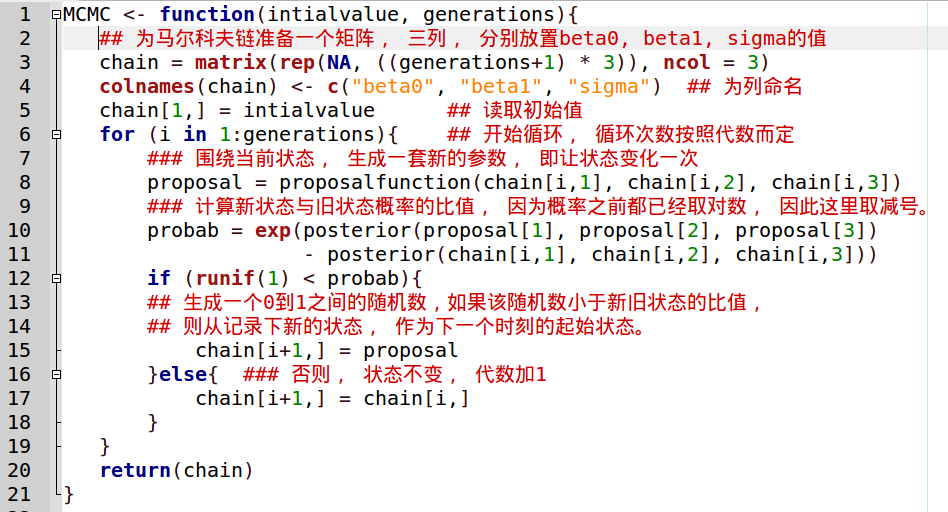
\includegraphics[height=2.6in]{Selection_070.png}\\
    \end{center}  
    \tt{
}
}


\frame{
    \frametitle{初始值不同的马尔科夫链}
    \tt{
初始值设定为 beta0 = 4, beta1 = 20, sigma = 1, 运行第一个马尔科夫链\\
res.chain1 $<-$ MCMC(intialvalue = c(4,20,1), generations = 100000) \\
    \medskip
初始值设定为 beta0 = 100, beta1 = 30, sigma =0.5, 运行第二个马尔科夫链\\
res.chain2 $<-$ MCMC(intialvalue = c(100,30,0.5), generations = 100000) \\
    \medskip
par(mfrow = c(1, 3))\\

plot(res.chain1[,1], res.chain1[,2], type = "l")  \\
随机取值点逐渐偏离初始值, 最后稳定在一个值附近\\
    \medskip
plot(res.chain1[,1], res.chain1[,3], type = "l")\\
plot(res.chain1[,2], res.chain1[,3], type = "l")\\
}
}

\frame{
    \frametitle{用coda程序包分析MCMC的结果}
         \begin{center}
    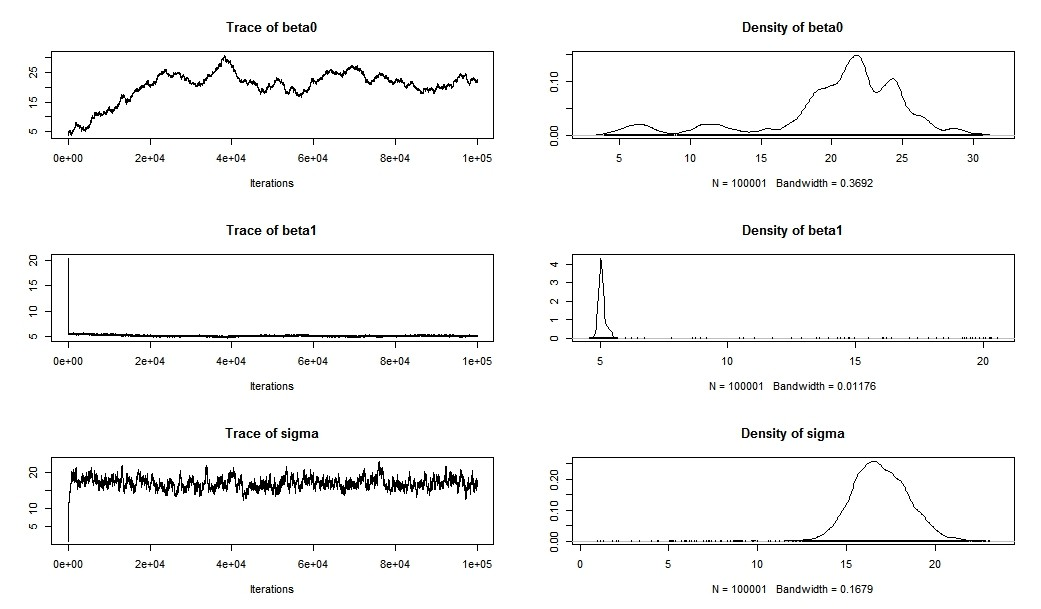
\includegraphics[height=2.2in]{coda.jpeg}\\
    \end{center}  
    
    \tt{
library(coda)\\
mcmc.res $<-$ mcmc(res.chain1)\\
summary(mcmc.res)\\
plot(mcmc.res)\\
}
}

\frame{
    \frametitle{分析MCMC的结果}
         \begin{center}
    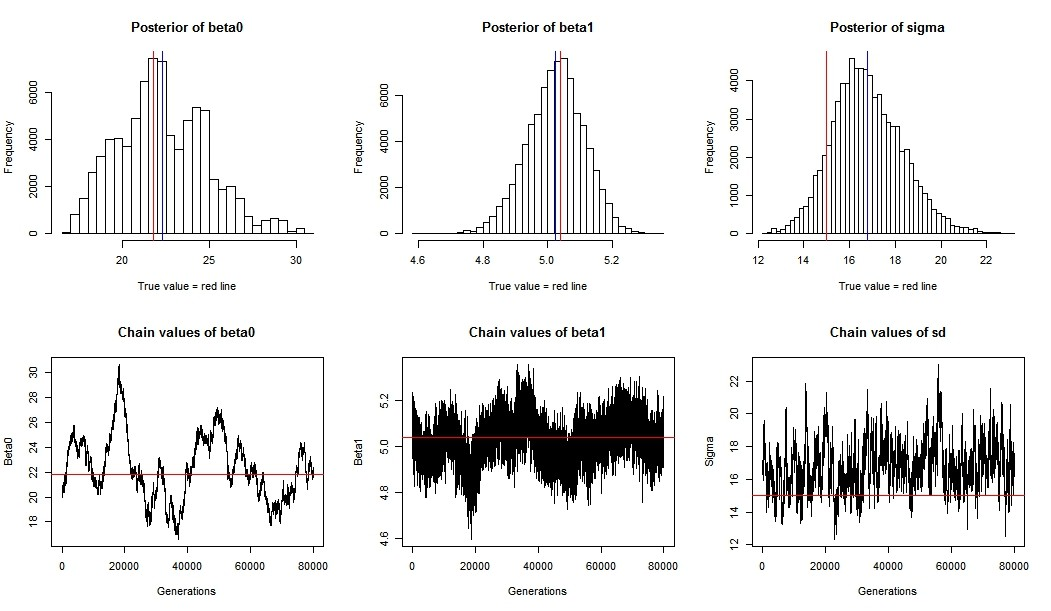
\includegraphics[height=2.2in]{mcmc_res.jpeg}\\
    \end{center}    
}

\frame{
    \frametitle{贝叶斯方法的在PCM的主要用途}
\begin{itemize}
\item 进化树推断
\item 祖先状态重建
\item 祖先分布区重建
\item 分化时间确定
\item 分化和灭绝速率的推断
\end{itemize}
}


\section{Bootstrap与Permutation Test}
\begin{frame}
\frametitle{目录}
\tableofcontents[currentsection] 
\end{frame}

\frame{
    \frametitle{Bootstrap从样本统计量估计总体统计量}
Bootstrap又称自展法,是用小样本估计总体值的一种非参数方法,在进化和生态学研究中应用十分广泛,例如, 进化树分化节点的自展支持率等。\\

Bootstrap的过程是生成一系列有放回随机抽样形成的伪样本。通过对伪样本的计算,获得统计量的分布。\\
\begin{block}{Bootstrap从样本求总体平均数}
例如,要进行1000次bootstrap,求平均值的置信区间,可以对每个伪样本计算平均值。这样就获得了1000个平均值。对这1000个平均值的分位数进行计算, 即可获得置信区间。已经证明,在初始样本足够大的情况下,bootstrap抽样能够无偏得接近总体的分布。
\end {block}
}

\frame{
    \frametitle{Bootstrap举例}
假设有一批产品,随机抽出30个,使用寿命(天数)如下,试用bootstrap的方法估计这批产品寿命95\%的置信区间。\\
\tt{
dat $<-$ c(119,120,131,209,210,337,332,287,146,\\
129,232,169,208,253,142,105,419,179,324,287,115,\\
132,308,356,286,221,204,105,45,245)\\
\medskip
\#\#\# 查看原始数据的频数直方图\\
hist(dat, col = "gray")\\
}

}

\frame{
    \frametitle{Bootstrap举例}
    
\begin{block}{Bootstrap求总体平均值的R代码}
\tt{
\#生成一个存储器\\
boot.sample $<-$ list()\\
\#\# 循环1000次,有放回的抽样,每次生成的\\
\#\# 新样本存储在boot.sample中\\
for(i in 1:1000)\{\\
     boot.sample{[[i]]} $<-$ sample(dat,size = 30, replace = TRUE)\\
\}\\
\#\# 求每个样本的mean,结果为1000个bootstrap样本的mean\\
boot.mean $<-$ unlist(lapply(boot.sample, mean))\\
\#\# 频数直方图\\
hist(boot.mean, col = "gray")\\
\#\# 求95\%的置信区间\\
CI95 $<-$ quantile(boot.mean, probs = c(0.025, 0.975))\\
\#\# 在频数直方图上加置信区间\\
abline(v = CI95, col = "red")\\
}
\end{block}

}

\frame{
    \frametitle{Permutation Test}
permutation 检验, 是检验某个统计量的实际值,是否偏离于随机分布的一种统计方法。 \\
方法为: 将真实数据随机排列后,生成一套随机数据, 根据该随机数据计算统计量。 \\
将这一步骤重复多次, 如999次, 基于随机数据的某个统计量的分布。 \\
将实际值和随机生成的统计量从小到达排列, 如果该统计量进入随机生成的统计量的95%的置信区间, 则该统计量不偏离于随机,即结果和随机并无差别。\\
 如果该统计量未能进入95%的置信区间, 则数据和随机在0.05的水平上有显著差异。\\

permutation test无需满足正态分布等假设, 即可做出统计推断。 是一种依据频率的非参数方法。用于检验community phylogenetic structure \\

}

\frame{
    \frametitle{问题}
极大似然法和贝叶斯方法有什么共同点?\\
你了解到的极大似然估计, 主要用在哪些领域?
}

\frame{
    \frametitle{进化树推断的方法}
\begin{itemize}
\item 1. 距离法:根据序列之间的遗传距离, 进行聚类分析。此方法基本上已经不用。 
\item 2. 最大简约法: 根据序列之间的位点差异, 找到一棵进化树, 并使该进化树上所发生的进化事件数目最少。 这种方法获得的进化树, 常用于极大似然法的起始树。
\item 3. 极大似然法: 在所有可能的进化树中, 找到最有可能形成当前序列的拓扑结构。 
\item 4. 贝叶斯法: 在所有可能的参数组合中, 随机给出若干参数的初始值,计算出Likelihood, 之后,让该参数组合随机变化, 并计算这种参数组合所发生的Likelihood, 将前后两次的Likelihood之比, 与0-1之间的随机数进行比较, 然后决定该参数组合的取舍。多次重复该过程后, 对所保留的参数进行汇总, 就得到进化树参数的分布, 即进化树。 
\end{itemize}
}

\frame{
    \frametitle{进化树推断的软件}
    R软件并不适于建立进化树, 而是用来分析所获得的进化树。 
\begin{itemize}
\item 1. 距离法:PHYLIP,PAUP*, ape 
\item 2. 最大简约法:PAUP*
\item 3. 极大似然法:PHYLIP, PAUP*, GARLI, RAxML, PHYML
\item 4. 贝叶斯法: MrBayes, BEAST, BayesPhy
\end{itemize}
}

\frame{
    \frametitle{中场休息: 问题?}
}

\end{document}
